%\begin{frame}
%    \centering
%    \Large{Part III:}\\
%    \ \\
%    \ \\
%    \centering
%    \Large{Real-space Density Functional Theory with\\ Localized Orbitals and Multiwavelets}
%\end{frame}

%\begin{frame}
%    \frametitle{The molecular Schr\"{o}dinger equation}
%    \ \\
%    \begin{equation}
%	\nonumber
%	\hat{H}\psi = E\psi
%    \end{equation}
%    \ \\
%    \begin{equation}
%	\nonumber
%	\hat{H} =   -\sum_I \frac{\nabla^2}{2M_I} - \sum_i \frac{\nabla^2}{2}
%		    +\sum_{I>J} \frac{Z_IZ_J}{|\boldsymbol{R}_I-\boldsymbol{R}_J|} 
%		    -\sum_{i,I} \frac{Z_I}{|\boldsymbol{r}_i-\boldsymbol{R}_I|} 
%		    +\sum_{i>j} \frac{1}{|\boldsymbol{r}_i-\boldsymbol{r}_j|} 
%    \end{equation}
%    \ \\
%    \ \\
%    \ \\
%    \centering
%    For an $N$-particle problem, the wave function is $3N$-dimensional
%    \begin{equation}
%	\nonumber
%	\psi = \psi(\boldsymbol{r}_1,\boldsymbol{r}_2,\dots,\boldsymbol{r}_N)
%    \end{equation}
%    \ \\
%    \ \\
%    \ \\
%    \pause
%    \centering
%    $\beta$-Carotene ($C_{40}H_{56}$) has 296 electrons and an 888-dimensional wave function!
%    \only<1>{
%    \begin{center}
%    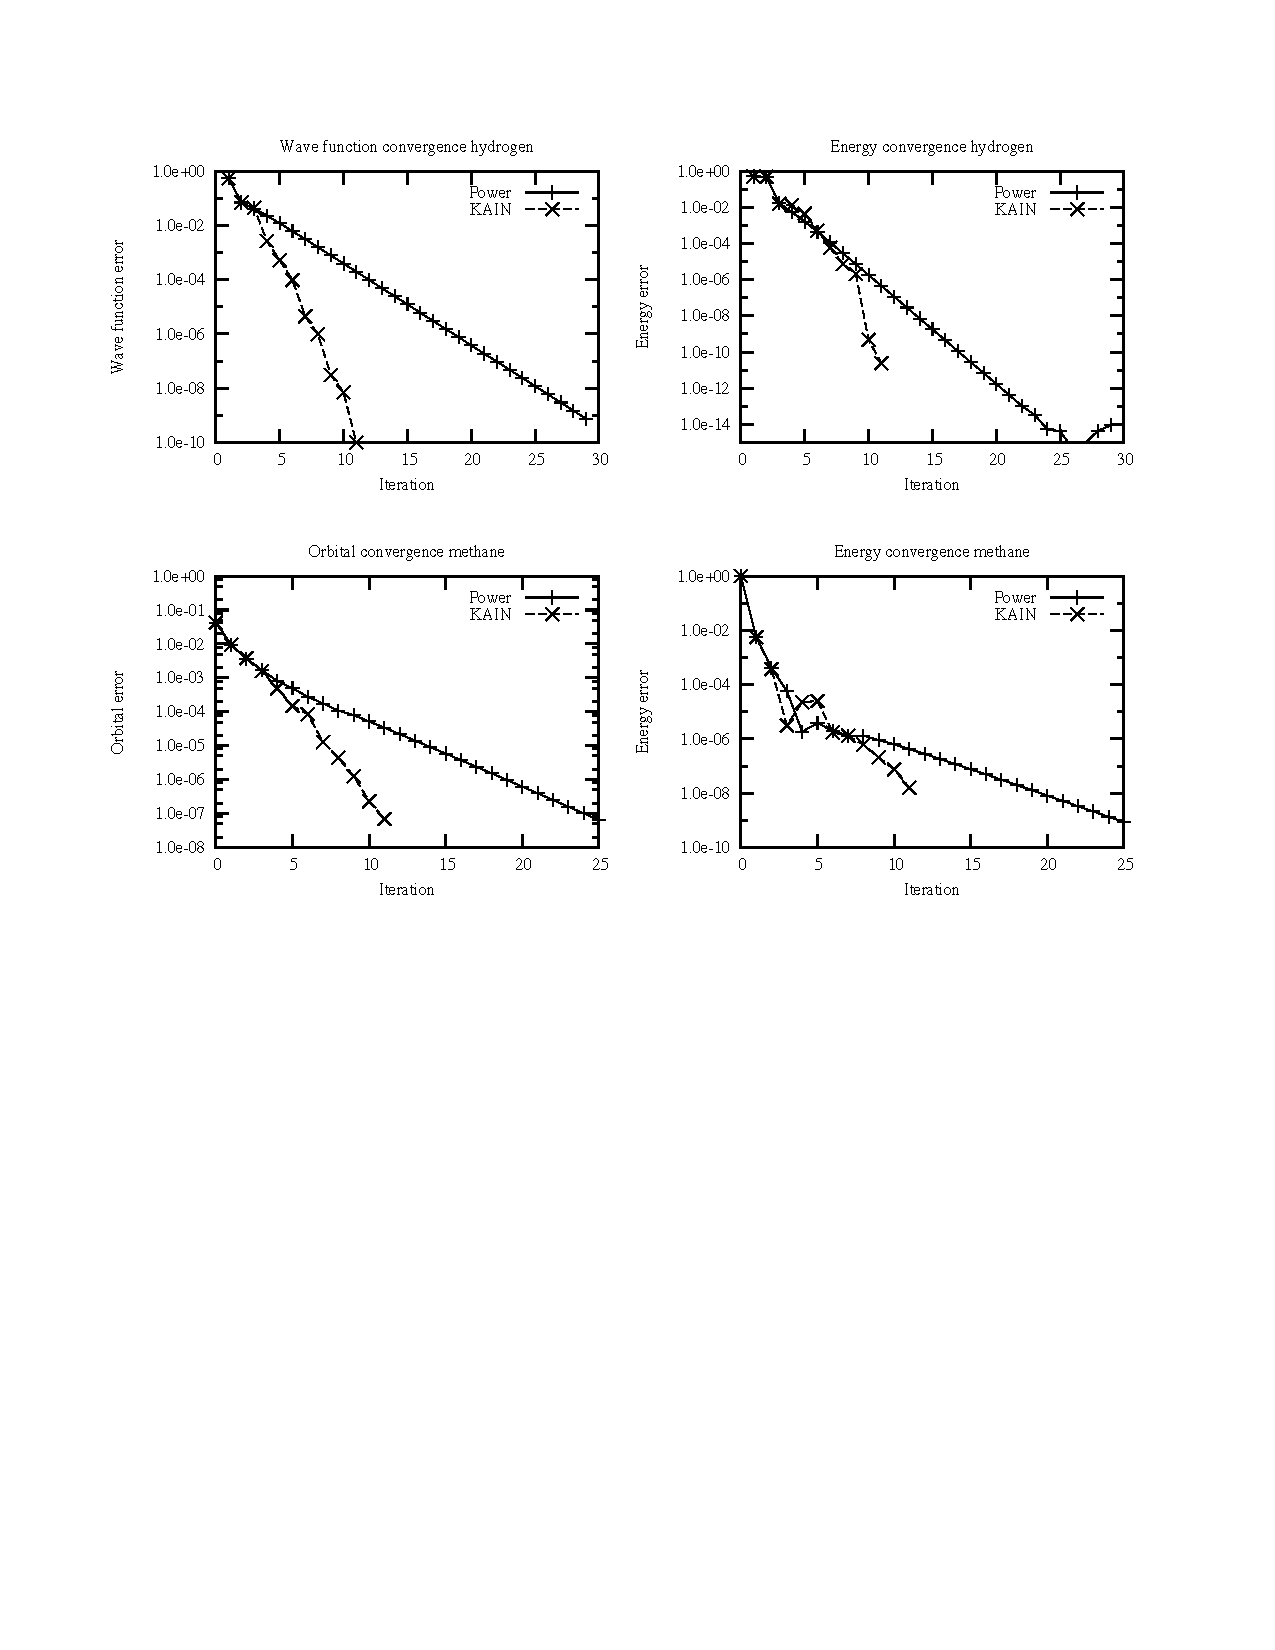
\includegraphics[scale=0.3, clip, viewport = 0 0 900 280]{figures/convergence.pdf}
%    \end{center}
%    }
%    \only<2>{
%    \begin{center}
%    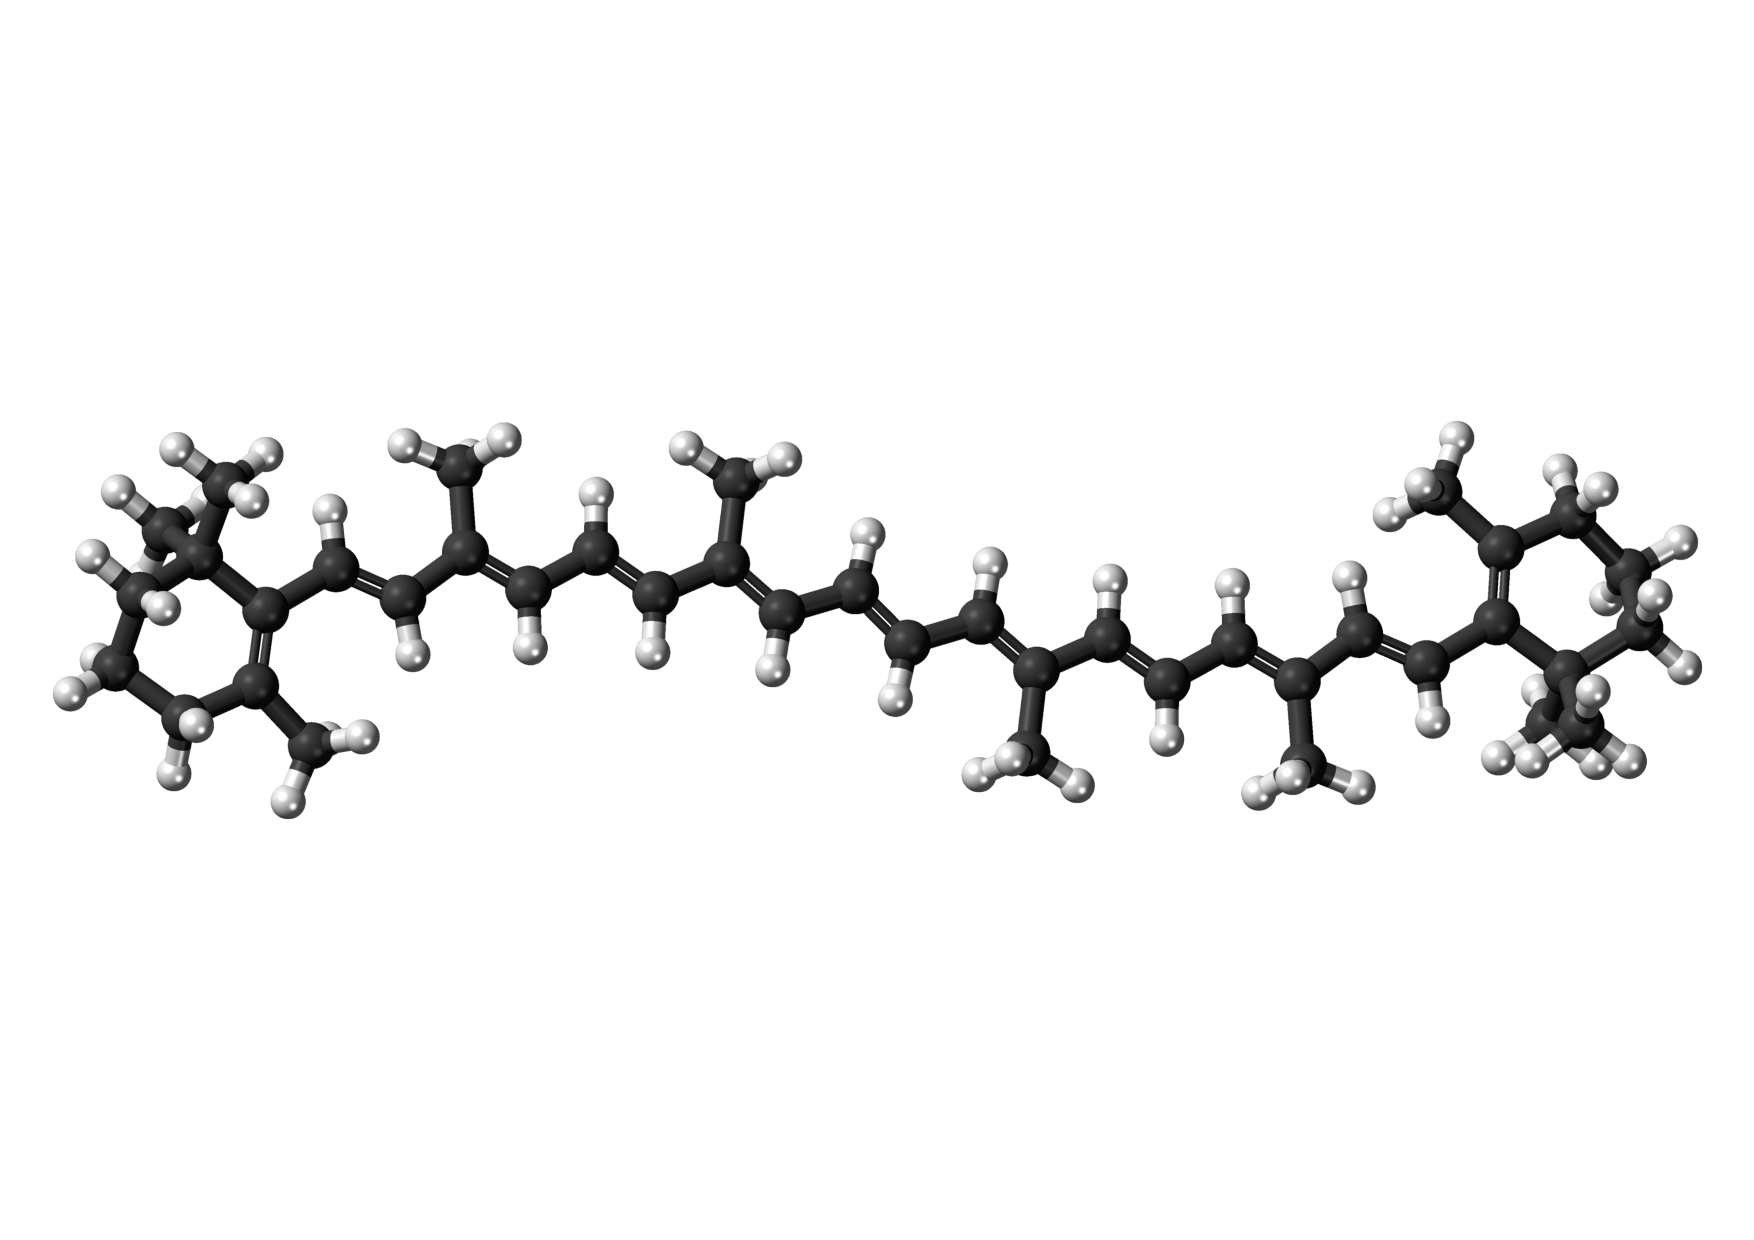
\includegraphics[scale=0.3, clip, viewport = 0 150 900 430]{figures/beta-carotene.pdf}
%    \end{center}
%    }
%\end{frame}

%\begin{frame}
%    \frametitle{Density Functional Theory}
%    \centering
%    Dramatically reduce the dimensionality
%    \begin{equation}
%	\nonumber
%	\rho(\boldsymbol{r}_1) = N \int |\psi(\boldsymbol{r}_1, \boldsymbol{r}_2,\dots,
%	\boldsymbol{r}_N)|^2 d\boldsymbol{r}_2\cdots d\boldsymbol{r}_N
%    \end{equation}
%    \ \\
%    \ \\
%    \ \\
%    \pause
%    Energy expressed as functional of the density
%    \begin{equation}
%	\nonumber
%	E[\rho] = T_s[\rho] + V_{ne}[\rho] + J[\rho] + E_{xc}[\rho]
%    \end{equation}
%    \ \\
%    \ \\
%    \ \\
%    \begin{columns}
%    \begin{column}{.50\textwidth}
%    \centering
%    \pause
%    \textbf{Energy expressions}
%    \begin{align}
%	\nonumber
%	V_{ne}[\rho]	&= \int \rho(\boldsymbol{r})v_{nuc}(\boldsymbol{r})d\boldsymbol{r}\\
%	\nonumber
%			&\\
%	\nonumber
%	J[\rho] &= \frac{1}{2} \int \rho(\boldsymbol{r})v_{el}(\boldsymbol{r})d\boldsymbol{r}\\
%	\nonumber
%			&\\
%	\nonumber
%	E_{xc}[\rho]	&= \int F_{xc}(\rho) d\boldsymbol{r}
%    \end{align}
%    \end{column}
%    \begin{column}{.50\textwidth}
%    \centering
%    \pause
%    \textbf{Potentials}
%    \begin{align}
%	\nonumber
%	v_{nuc}(\boldsymbol{r}) &= -\sum_I\frac{Z_I}{|\boldsymbol{r}-\boldsymbol{R}_I|}\\
%	\nonumber
%			&\\
%	\nonumber
%	v_{el}(\boldsymbol{r}) &= 
%	    \int \frac{\rho(\boldsymbol{r}')}{4\pi|\boldsymbol{r}-\boldsymbol{r}'|} d\boldsymbol{r}'\\
%	\nonumber
%			&\\
%	\nonumber
%	v_{xc}(\boldsymbol{r}) &= \frac{\delta E_{xc}[\rho]}{\delta\rho}
%    \end{align}
%    \end{column}
%    \end{columns}    
%\end{frame}

%\begin{frame}
%    \frametitle{Kohn-Sham DFT}
%    \centering
%    Express density through one-electron orbitals
%    \begin{equation}
%	\nonumber
%	\rho(\boldsymbol{r}) = \sum_i |\phi_i(\boldsymbol{r})|^2
%    \end{equation}
%    \ \\
%    \ \\
%    \ \\
%    \ \\
%    \pause
%    \begin{columns}
%    \begin{column}{.50\textwidth}
%    \centering
%    Kinetic energy
%    \begin{equation}
%	\nonumber
%	T_s[\rho] = -\sum_i \frac{1}{2}\nabla^2\phi_i(\boldsymbol{r})
%    \end{equation}
%    \end{column}
%    \begin{column}{.50\textwidth}
%    \centering
%    Effective potential
%    \begin{equation}
%	\nonumber
%	v_{eff}(\boldsymbol{r}) = v_{nuc}(\boldsymbol{r}) + v_{el}(\boldsymbol{r}) + v_{xc}(\boldsymbol{r})
%    \end{equation}
%    \end{column}
%    \end{columns}
%    \ \\
%    \ \\
%    \ \\
%    \ \\
%    \pause
%    \centering
%    \textbf{The Kohn-Sham equations}
%    \begin{equation}
%	\nonumber
%	\left[-\frac{1}{2}\nabla^2 + v_{eff}(\boldsymbol{r})\right]\phi_i(\boldsymbol{r}) = 
%	\epsilon_i\phi_i(\boldsymbol{r})
%    \end{equation}
%\end{frame}

\begin{frame}
    \frametitle{Computational chemistry}
    \begin{center}
%    \only<1>{\includegraphics[scale=0.5, clip, viewport = 50 300 550 800]
%        {figures/basis_set_1.pdf}}
%    \only<2>{\includegraphics[scale=0.5, clip, viewport = 50 300 550 800]
%        {figures/basis_set_2.pdf}}
    \only<1>{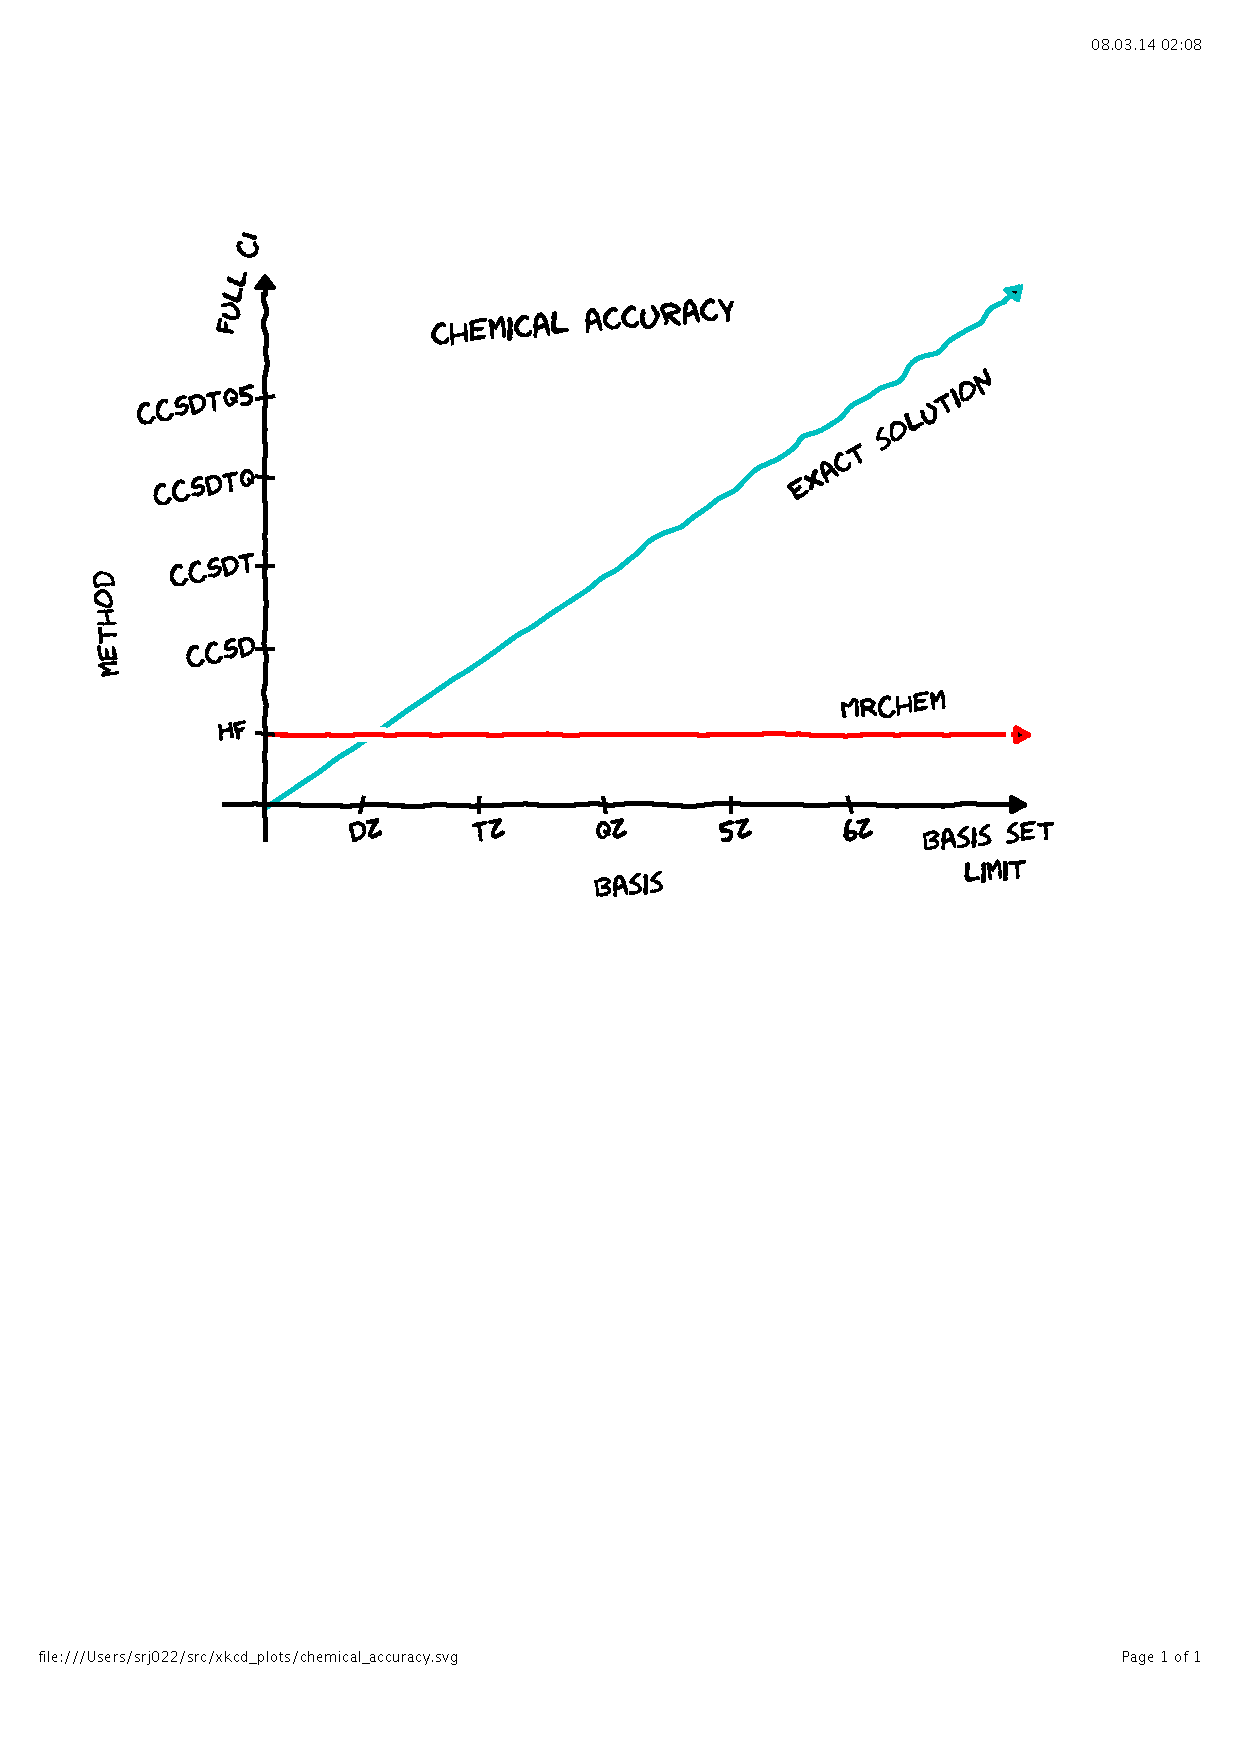
\includegraphics[scale=0.5, clip, viewport = 0 300 550 800]
        {figures/chemical_accuracy.pdf}}
    \end{center}
\end{frame}


